\documentclass[a4j]{jarticle}
\usepackage{ascmac}
\usepackage[dvipdfmx]{graphicx}
\usepackage{listings}

\lstset{
  basicstyle={\ttfamily},
  identifierstyle={\small},
  commentstyle={\smallitshape},
  keywordstyle={\small\bfseries},
  ndkeywordstyle={\small},
  stringstyle={\small\ttfamily},
  frame={tb},
  breaklines=true,
  columns=[l]{fullflexible},
  numbers=left,
  xrightmargin=0zw,
  xleftmargin=3zw,
  numberstyle={\scriptsize},
  stepnumber=1,
  numbersep=1zw,
  lineskip=-0.5ex
}
\renewcommand{\lstlistingname}{ソースコード}

\begin{document}

\title{計算機科学実験及演習1 報告書 \\ \bf 課題12}
% ↓ここに自分の氏名を記入
\author{安済 翔真}
\西暦
\date{提出日: \today} % コンパイル時の日付が自動で挿入される
\maketitle

\section{最短経路探索アルゴリズム}
\subsection{アルゴリズムの説明}
以下に、実装したダイクストラ法のアルゴリズムを示す。
\begin{enumerate}
  \item 距離が確定した頂点の集合A、始点から頂点vまでの距離を返す関数D(v)、
  最短経路において頂点vの1つ前に通る頂点を返す関数P(v)、少なくとも1回訪れた頂点の集合Q、
  頂点\(v, w\)間の辺の重みを返す関数\(W(v, w)\)を用意する。
  はじめは\(\forall v \in V(頂点全体の集合), D(v) = \infty \)としておく。
  \item 始点\(v_0\)からの距離\(D(v_0) = 0\)とする。また、Qに\(v_0\)を追加する。
  \item Qの要素数が0になるまで以下を繰り返す。
    \begin{enumerate}
      \item Qの要素の中で、始点からの距離が最小の要素vを取り出す。
      \item vに隣接する各頂点wに対して、\(D(w) > D(v) + W(v, w)\)ならば
      \(D(w) = D(v) + W(v, w)\)とし、\(Qにw\)を追加する。また、\(P(w) = v\)とする。
    \end{enumerate}
\end{enumerate}
以上の操作によって定められた\(P(v)\)の値を辿ることで始点から任意の点までの最短経路を求めることができる。

\newpage
\subsection{アルゴリズムの流れ図}
% 次の3行のコメントをはずし,図のファイル名,拡大縮小率を調整する.
\begin{figure}[h]
  \centering
  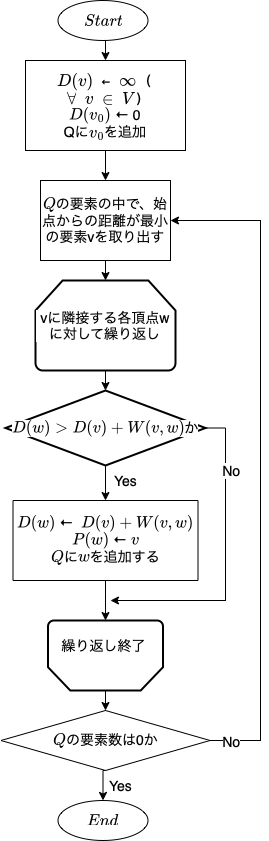
\includegraphics[scale=0.5]
    {report12.drawio.png}
\end{figure}

\subsection{実行例}
% MyGraphTestの典型的な実行例(端末からの入力や出力を含む)を示す.
% {screen}環境を使うと,枠を出力できる.

\begin{screen}
\$ java MyGraphTest \\
graph.txt  \\
3
\end{screen}

\section{クラス仕様}
この章では実装したクラスの仕様を説明する。
% クラス仕様とは,そのクラスが持つ役割,
% メンバ変数,メソッドなどの仕様を記述したものである.
% 本レポートでは,自身が作成したクラス
%(MyGraphやMyEdgeなど)それぞれについて,
% subsectionを作成し,クラス仕様を記述すること

\subsection{MyEdgeクラス}

\subsubsection{役割}
% このクラスが持つ役割を簡潔に数行で記述する.
このクラスはグラフ内の辺を表す。辺の両端の頂点と辺の重みを変数として保持し、このクラスのインスタンス
メソッドを呼び出すことでそれらを取得することができる。

\subsubsection{メンバ変数}
%クラスが持つすべてのメンバ変数について,descriptionで記述

\begin{description}
\item[Integer node1]
辺の両端の頂点のうち、頂点番号が小さい方の頂点の番号を保持する。

\item[Integer node2]
辺の両端の頂点のうち、頂点番号が大きい方の頂点の番号を保持する。

\item[Integer weight]
辺の重みを保持する。

\end{description}

%クラスが持つすべてのメソッドについて,subsubsectionを作り,説明
\subsubsection{getNodesメソッド}

\begin{description}
\item[機能]
辺の両端の頂点番号を配列として返す。

\item[インタフェース]\ \vspace{0mm}
\begin{enumerate}
  \item 引数: なし
  \item 返り値の型: Integer[]
\end{enumerate}
\end{description}

\subsubsection{getWeight}

\begin{description}
\item[機能]
辺の重みを返す。

\item[インタフェース]\ \vspace{0mm}
\begin{enumerate}
  \item 引数: なし
  \item 返り値の型: Integer[]
\end{enumerate}
\end{description}

\subsection{MyGraphクラス}

\subsubsection{役割}
このクラスはグラフそのものを表す。入力ファイルからグラフを読み取って辺をリストとして保持する。
グラフに対する種々の操作を行うためのメソッドが用意されている。

\subsubsection{メンバ変数}

\begin{description}
\item[final int MAX\_NODES\_NUM]
許容可能な頂点の個数の最大値を表す。

\item[final int MAX\_EDGES\_NUM]
許容可能な辺の個数の最大値を表す。

\item[final integer MAX\_WEIGHT]
許容可能な辺の重みの最大値を表す。

\item[final integer MIN\_WEIGHT]
許容可能な辺の重みの最小値を表す。

\item[LinkedList\textless MyEdge\textgreater[] ]
許容可能な辺の重みの最小値を表す。

\end{description}

%クラスが持つすべてのメソッドについて,subsubsectionを作り,説明
\subsubsection{readFromFileメソッド}

\begin{description}
\item[機能]
入力ファイルからグラフを読み取って辺をリストとして保持する

\item[インタフェース]\ \vspace{0mm}
\begin{enumerate}
  \item 引数: String filename
  \item 返り値: なし
\end{enumerate}
\end{description}

\subsubsection{getEdgesメソッド}

\begin{description}
\item[機能]
引数に与えられた頂点につながる辺のリストを返す。

\item[インタフェース]\ \vspace{0mm}
\begin{enumerate}
  \item 引数: int id
  \item 返り値の型: LinkedList\textless MyEdge\textgreater
\end{enumerate}
\end{description}

\subsubsection{getLinkedNodesメソッド}

\begin{description}
\item[機能]
引数に与えられた頂点につながる頂点の配列を返す。

\item[インタフェース]\ \vspace{0mm}
\begin{enumerate}
  \item 引数: int id
  \item 返り値の型: Integer[]
\end{enumerate}
\end{description}

\subsubsection{getWeightメソッド}

\begin{description}
\item[機能]
引数に与えられた2つの頂点の間の辺の重みを返す。

\item[インタフェース]\ \vspace{0mm}
\begin{enumerate}
  \item 引数: Integer v, Integer w
  \item 返り値の型: Integer
\end{enumerate}
\end{description}

\subsubsection{getNodeSizeメソッド}

\begin{description}
\item[機能]
グラフ内の頂点の個数を返す。

\item[インタフェース]\ \vspace{0mm}
\begin{enumerate}
  \item 引数: なし
  \item 返り値の型: int
\end{enumerate}
\end{description}

\subsubsection{getShortestPathメソッド}

\begin{description}
\item[機能]
ダイクストラ法により始点から終点までの最短経路を求める。
返り値には、始点から拡張点に至るまでのパスにおいて、各頂点の1つ前の頂点番号が格納された配列が返される。

\item[インタフェース]\ \vspace{0mm}
\begin{enumerate}
  \item 引数: Integer start, Integer end
  \item 返り値の型: Integer[]
\end{enumerate}
\end{description}

\subsection{Nodeクラス}

\subsubsection{役割}
% このクラスが持つ役割を簡潔に数行で記述する.
このクラスは頂点そのものを表す。ダイクストラ法において、すでに訪れた頂点の集合\(found\)の中から
始点からの距離が最も小さい頂点を取り出す際、通常の配列を用いると\(O(n)\)かかってしまうため、\(PriorityQueue\)
を用いて実装をした。ヒープは始点からの距離を基準として構成する必要があるため、頂点の大小を
始点からの距離で測るよう\(compareTo\)メソッドが\(Override\)して実装されている。

\subsubsection{メンバ変数}
%クラスが持つすべてのメンバ変数について,descriptionで記述

\begin{description}
\item[Integer id]
頂点番号を保持する。

\item[Integer distance]
始点からの距離を保持する。

\end{description}

%クラスが持つすべてのメソッドについて,subsubsectionを作り,説明
\subsubsection{compareToメソッド}

\begin{description}
\item[機能]
頂点の順序関係を表す。自身と引数で与えられた頂点を比べて、始点からの距離が自身の方が小さければ
負の値を、大きければ正の値を返し、等しければ0を返す。

\item[インタフェース]\ \vspace{0mm}
\begin{enumerate}
  \item 引数: Node node
  \item 返り値の型: int
\end{enumerate}
\end{description}

\subsection{MyGraphTestクラス}

\subsubsection{役割}
% このクラスが持つ役割を簡潔に数行で記述する.
このクラスは、MyGraphクラスのgetShortestPathメソッドをテストするのに用いる。

\subsubsection{メンバ変数}
%クラスが持つすべてのメンバ変数について,descriptionで記述
なし。

%クラスが持つすべてのメソッドについて,subsubsectionを作り,説明
\subsubsection{mainメソッド}

\begin{description}
\item[機能]
MyGraphクラスの\(getShortestPath\)をテストする。
標準入力から、入力ファイルの名前と始点・終点の頂点番号を受け取り、始点から終点までの最短経路と
それにかかるコストを標準出力に出力する。


\item[インタフェース]\ \vspace{0mm}
\begin{enumerate}
  \item 引数: String[] args
  \item 返り値の型: なし
\end{enumerate}
\end{description}


\section{プログラムの評価}

% 以下のような点について自由記述.
% ・採用した設計,論理に関する検討(代替案との比較)
% ・プログラムの作成にあたって創意工夫した点
% ・テストの十分性(すべてのプログラムパスを網羅しているか)
% ・完成に至るまでに発生したバグの現象とその処置
% ・プログラムの機能的完成度(改良,拡張の余地)
% ・プログラムの効率
% ・その他

本プログラムにおいて工夫した点は、すでに訪れた頂点の集合を表す\(found\)を\(PriorityQueue\)で
表すことで、\(found\)の中で始点からの距離が最も小さい頂点を取り出すのにかかる時間を\(O(\log n)\)に
抑えたことである。ヒープは始点からの距離を基準として構成する必要があるため、Nodeクラスを用意し、
\(compareTo\)メソッドをOverrideすることで頂点の順序関係を自身で作成した。これによりプログラム全体の
計算量は\(O(n\log n)\ (n: 頂点の個数)\)程度に抑えられている。
テストにおいては、連結グラフにおいて正しくパスが出力されること・入力ファイルに不適切な文字が入って
いた場合に正常に例外処理をしてプログラムを終了すること・始点と終点が繋がっていなかった場合に正常に終了する
ことを確認した。

\section{プログラム開発の経過}

% プログラム開発の各段階で要した時間配分(工数)の概略を記す.
% あともどりがあった場合はその状況についても説明する.
% 各段階とは次の通り:
% 1. 問題の分析と解法の検討
% 2. クラス設計(クラスにどんなメソッドを用意するか設計すること)
% 3. クラス内論理設計/プログラミング(各メソッドを実際に実装すること)
% 4. プログラムテスト,デバッグ
% 5. 仕様書の作成(このレポートの作成)
\begin{enumerate}
  \item 問題の分析と解法の検討\\
  課題12のwikiを読んで要求仕様を確認した。この段階には、
  ダイクストラ法のアルゴリズムの確認などを含めて1時間ほど費やした。
  \item クラス設計\\
  \(PriorityQueue\)を用いるのに必要なNodeクラスの設計などに時間がかかり、2時間ほど費やした。
  \item クラス内論理設計\\
  約1時間。
  \item プログラムテスト・デバッグ\\
  約30分。
  \item 仕様書の作成\\
  約5時間。
\end{enumerate}

\section{感想}

% 自由記述.
% シラバスに示した参考書以外のものを参照した場合,それも記す.
入力ファイルに不適切な文字が含まれていた場合の例外処理を考えるのに苦労した。
また、計算量を抑えるために、\(found\)を\(PriorityQueue\)で表すために、Nodeクラスを
作成して\(compareTo\)メソッドをOverrideするというのが難しく、時間がかかった。グラフの
表し方は他にもあるそうなので、別の表し方でプログラムを書くことも試してみたいと感じた。

\newpage
\section*{付録}

% 作成したすべてのクラスのソースコードをつける.
% \ver
\begin{lstlisting}[caption=MyEdge.java]
public class MyEdge {
    private Integer node1;
    private Integer node2;
    private Integer weight;

    public MyEdge(Integer node1, Integer node2, Integer weight) {
        this.node1 = Math.min(node1, node2);
        this.node2 = Math.max(node1, node2);
        this.weight = weight;
    }

    public Integer[] getNodes() {
        Integer[] nodes = { this.node1, this.node2 };
        return nodes;
    }

    public Integer getWeight() {
        return this.weight;
    }
}

\end{lstlisting}

\begin{lstlisting}[caption=Node.java]
public class Node implements Comparable<Node> {
    Integer id;
    Integer distance;

    public Node(Integer id, Integer distance) {
        this.id = id;
        this.distance = distance;
    }

    @Override
    public int compareTo(Node node) {
        return this.distance - node.distance;
    }
}
\end{lstlisting}

\begin{lstlisting}[caption=MyGraph.java]
import java.io.File;
import java.io.FileNotFoundException;
import java.util.Arrays;
import java.util.LinkedList;
import java.util.PriorityQueue;
import java.util.Scanner;

public class MyGraph {
    private final int MAX_NODES_NUM = 50;
    private final int MAX_EDGES_NUM = 100;
    private final Integer MAX_WEIGHT = 9999;
    private final Integer MIN_WEIGHT = 1;

    private LinkedList<MyEdge>[] edges;

    public void readFromFile(String filename) {
        try {
            File file = new File(filename);
            Scanner scanner = new Scanner(file);
            int nodeNum = Integer.parseInt(scanner.nextLine());
            int edgeNum = Integer.parseInt(scanner.nextLine());

            if (nodeNum > MAX_NODES_NUM) {
                String message = String.format(
                    "The number of nodes must be less than %d.",
                    MAX_NODES_NUM
                );
                scanner.close();
                throw new RuntimeException(message);
            }
            if (edgeNum > MAX_EDGES_NUM) {
                String message = String.format(
                        "The number of edges must be less than %d.",
                        MAX_EDGES_NUM);
                scanner.close();
                throw new RuntimeException(message);
            }

            this.edges = new LinkedList[nodeNum];

            for (int i = 0; i < nodeNum; i++) {
                this.edges[i] = new LinkedList<MyEdge>();
            }
            for (int i = 0; i < edgeNum; i++) {
                String[] chars = scanner.nextLine().split(" ");
                Integer[] nums = new Integer[chars.length];

                for (int j = 0; j < chars.length; j++) {
                    nums[j] = Integer.parseInt(chars[j]);
                }

                if (nums[2] > MAX_WEIGHT || nums[2] < MIN_WEIGHT) {
                    String message = String.format(
                        "The weight value must be between %d and %d.",
                        MIN_WEIGHT, MAX_WEIGHT
                    );
                    scanner.close();
                    throw new RuntimeException(message);
                }

                this.edges[nums[0]].add(new MyEdge(nums[0], nums[1], nums[2]));
                this.edges[nums[1]].add(new MyEdge(nums[0], nums[1], nums[2]));
            }

            scanner.close();
        }
        catch (FileNotFoundException ex) {
            System.out.println("File not found.");
            System.exit(0);
        }
        catch (NumberFormatException ex) {
            System.out.println("Input must be an integer value.");
            System.exit(0);
        }
        catch (RuntimeException ex) {
            System.out.println(ex.getMessage());
            System.exit(0);
        }
    }

    public LinkedList<MyEdge> getEdges(int id) {
        return this.edges[id];
    }

    private Integer[] getLinkedNodes(int id) {
        LinkedList<MyEdge> edges = this.getEdges(id);
        Integer[] nodes = new Integer[edges.size()];
        for (int i = 0; i < edges.size(); i++) {
            Integer[] ends = edges.get(i).getNodes();
            nodes[i] = ends[0] == id ? ends[1] : ends[0];
        }

        return nodes;
    }

    public Integer getWeight(Integer v, Integer w) {
        LinkedList<MyEdge> edges = this.getEdges(v);
        for (MyEdge edge : edges) {
            if (Arrays.asList(edge.getNodes()).contains(w)) {
                return edge.getWeight();
            }
        }
        String message = String.format("The vertices %s and %s are not connected.", v, w);
        throw new RuntimeException(message);
    }

    private int getNodeSize() {
        return this.edges.length;
    }

    public Integer[] getShortestPath(Integer start, Integer end) {
        int size = this.getNodeSize();
        boolean[] determined = new boolean[size];
        Integer[] distances = new Integer[size];
        Integer[] prevs = new Integer[size];

        PriorityQueue<Node> found = new PriorityQueue<>();

        for (int i = 0; i < size; i++) {
            distances[i] = Integer.MAX_VALUE;
        }
        distances[start] = 0;

        found.add(new Node(start, 0));

        while (true) {
            if (found.size() == 0) {
                break;
            }

            Node node = found.poll();
            int minId = node.id;
            
            if (determined[minId]) {
                continue;
            }
            determined[minId] = true;

            for (int nextId : this.getLinkedNodes(minId)) {
                if (distances[nextId] > distances[minId] + this.getWeight(minId, nextId)) {
                    distances[nextId] = distances[minId] + this.getWeight(minId, nextId);
                    found.add(new Node(nextId, distances[nextId]));
                    prevs[nextId] = minId;
                }
            }
        }

        return prevs;
    }
}
\end{lstlisting}

\begin{lstlisting}[caption=MyGraphTest.java]
import java.util.ArrayList;
import java.util.InputMismatchException;
import java.util.NoSuchElementException;
import java.util.Scanner;

public class MyGraphTest {
    public static void main(String[] args) {
        try {
            Scanner scanner = new Scanner(System.in);
            String filename = scanner.nextLine();
            int start = Integer.parseInt(scanner.nextLine());
            int end = Integer.parseInt(scanner.nextLine());
            scanner.close();

            MyGraph graph = new MyGraph();
            graph.readFromFile(filename);

            Integer[] prevs = graph.getShortestPath(start, end);
            Integer point = end;
            Integer weightSum = 0;
            ArrayList<Integer> path = new ArrayList<>();
            path.add(0, end);

            while (true) {
                if (point == start) {
                    break;
                }

                if (prevs[point] == null) {
                    String message = "The start and end points are not connected.";
                    throw new RuntimeException(message);
                }
                weightSum += graph.getWeight(point, prevs[point]);
                point = prevs[point];
                path.add(0, point);
            }

            for (int i = 0; i < path.size(); i++) {
                System.out.print(path.get(i));
                if (i == path.size() - 1) {
                    System.out.print("\n");
                }
                else {
                    System.out.print(" ");
                }
            }
            System.out.println(weightSum);
        }
        catch (InputMismatchException ex) {
            System.out.println(ex.getMessage());
            System.exit(0);
        }
        catch (NoSuchElementException ex) {
            System.out.println("The actual number of edges given is less than the number of edges specified in the file.");
            System.exit(0);
        }
        catch (RuntimeException ex) {
            System.out.println(ex.getMessage());
            System.exit(0);
        }
    }
}  
\end{lstlisting}

\end{document}
